% ============================================================
% Final Project Presentation
% Project 01: Sign Language Translation (signlang)
% Course: CSC15012 - Applications of NLP in Industry
% Student: Le Dinh Minh Quan - 23127460 - 23CNTThuc
% Template based on Madrid + seahorse (Overleaf Beamer)
% ============================================================

\documentclass[10pt,aspectratio=169]{beamer}

\mode<presentation>
{
  \usetheme{Madrid}
  \usecolortheme{seahorse}
  \usefonttheme{default}
  \setbeamertemplate{navigation symbols}{}
  \setbeamertemplate{caption}[numbered]
  \setbeamertemplate{footline}[frame number]
}

% ---- Packages ----
\usepackage[english]{babel}
\usepackage[utf8]{inputenc}
\usepackage{amsmath}
\usepackage{amssymb}
\usepackage{graphicx}
\usepackage{booktabs}
\usepackage{xcolor}
\usepackage{hyperref}
\usepackage{xurl}
\usepackage{tikz}
\usepackage{pgfplots}
\pgfplotsset{compat=1.18}
\usetikzlibrary{shapes.geometric, arrows.meta, positioning, fit, backgrounds, shadows}
\usepackage{listings}
\lstset{
  basicstyle=\ttfamily\scriptsize,
  breaklines=true,
  frame=single,
  backgroundcolor=\color{gray!10},
  keywordstyle=\color{blue},
  commentstyle=\color{green!60!black},
  stringstyle=\color{red!70!black},
  showstringspaces=false,
  tabsize=2
}

% ---- HCMUS LOGO ----
% Upload logo_hcmus.png to Overleaf to display the logo (top-right of every slide).
% If the file is missing, no logo is shown (no error).
\IfFileExists{logo_hcmus.png}{\logo{\includegraphics[height=0.7cm]{logo_hcmus.png}}}{}

% ---- TITLE METADATA ----
\title[Project 01: Sign Language Translation]{Project 01: Sign Language Translation}
\subtitle{A Sign2Gloss2Text Cascade with a 5-Decision Abstaining Agent}
\author[Le Dinh Minh Quan]{Le Dinh Minh Quan \\ \small ID: 23127460 -- Class: 23CNTThuc}
\institute[HCMUS]{Vietnam National University Ho Chi Minh City \\ University of Science -- Faculty of Information Technology \\ \small Course: CSC15012 -- Applications of NLP in Industry}
\date{2026}

\begin{document}

% ============================================================
% SLIDE 1: TITLE
% ============================================================
\begin{frame}
  \titlepage
\end{frame}

% ============================================================
% SLIDE 2: OUTLINE
% ============================================================
\begin{frame}{Outline}
\begin{columns}[T]
\begin{column}{0.5\textwidth}
\begin{enumerate}
  \item Business Problem \& Motivation
  \item Proposed NLP Solution \& Success Metrics
  \item System Architecture
  \item Repository \& Tech Stack
  \item Data Management
  \item Training \& Autopilot Workflow
  \item Evaluation Results
\end{enumerate}
\end{column}
\begin{column}{0.5\textwidth}
\begin{enumerate}
  \setcounter{enumi}{7}
  \item The 5-Decision Agent
  \item Agent Example Traces
  \item Deployment
  \item Ethics, Privacy \& Fairness
  \item Monitoring \& Continual Learning
  \item Key Takeaways \& Future Work
  \item Resources \& Thank You
\end{enumerate}
\end{column}
\end{columns}
\end{frame}

% ============================================================
% SLIDE 3: BUSINESS PROBLEM & MOTIVATION
% ============================================================
\begin{frame}{1. Business Problem \& Motivation}
\begin{block}{Context}
Sign Language Translation maps a signed-language \textbf{video / pose sequence} into spoken-language \textbf{text}. Deaf/hard-of-hearing access to spoken services needs interpreters who are not always available -- an \textbf{assistive} tool can bridge gaps, caption signed media, and serve fixed-vocabulary kiosks.
\end{block}

\begin{columns}[T]
\begin{column}{0.5\textwidth}
\textbf{Why it is hard}
\begin{itemize}
  \item Continuous (co-articulated) signing $\Rightarrow$ must \textbf{segment} first
  \item Signer-independence: a model on one signer fails on others
  \item \textbf{Restrictive licensing} -- every continuous SLT corpus is NC / gated / unspecified
  \item No loadable Sign$\rightarrow$Text checkpoint on the Hub
  \item OOV signs $\Rightarrow$ blind decoders \textbf{hallucinate}
\end{itemize}
\end{column}
\begin{column}{0.5\textwidth}
\textbf{Stakeholders}
\begin{itemize}
  \item Deaf / hard-of-hearing signers
  \item Hearing participants (draft transcript)
  \item Qualified interpreters (human-in-the-loop)
  \item Developers \& researchers (REST API)
\end{itemize}
\textbf{Why NLP}: signed languages are real \emph{translation} (reordering + lexicon), not transcription.
\end{column}
\end{columns}
\end{frame}

% ============================================================
% SLIDE 4: PROPOSED NLP SOLUTION + SUCCESS METRICS
% ============================================================
\begin{frame}{2. Proposed NLP Solution \& Success Metrics}
\begin{block}{Solution}
A \textbf{Sign2Gloss2Text cascade}: frozen pose front-end $\rightarrow$ motion segment $\rightarrow$ gloss recognizer (trained) $\rightarrow$ gloss$\rightarrow$text translator (trained) $\rightarrow$ a deterministic \textbf{5-decision agent} (D1--D5) that gates confidence, verifies, and \textbf{abstains}. Runs fully offline on a synthetic pose generator; upgrades to MediaPipe + transformer + \texttt{t5-small} on Colab.
\end{block}

\begin{table}[h]
\centering\small
\begin{tabular}{lll}
\toprule
\textbf{Stage} & \textbf{Metric} & \textbf{Target (offline synthetic)} \\
\midrule
Recognition & Gloss accuracy / WER / exact-match & $\gg$ floor 0.02 / $\rightarrow$0 / high \\
Segmentation & Boundary-F1 & $\rightarrow$ 1.0 \\
Translation & BLEU-4 (headline) / chrF & beat identity $\approx$84 \\
Agent & Abstention rate & $\approx$0 clean $\rightarrow$ $\approx$1 noise \\
\bottomrule
\end{tabular}
\end{table}

\textbf{Result preview} (verified offline): gloss accuracy \textbf{1.0}, BLEU \textbf{99+}, segmentation-F1 \textbf{1.0} vs most-frequent floor \textbf{0.02} / identity-translate \textbf{$\approx$84} BLEU; pure-noise input \textbf{abstains}; rubric self-check \textbf{score 1.0}.
\end{frame}

% ============================================================
% SLIDE 5: SYSTEM ARCHITECTURE (TikZ)
% ============================================================
\begin{frame}{3. System Architecture (Sign2Gloss2Text Cascade)}
\centering
\resizebox{0.96\linewidth}{!}{%
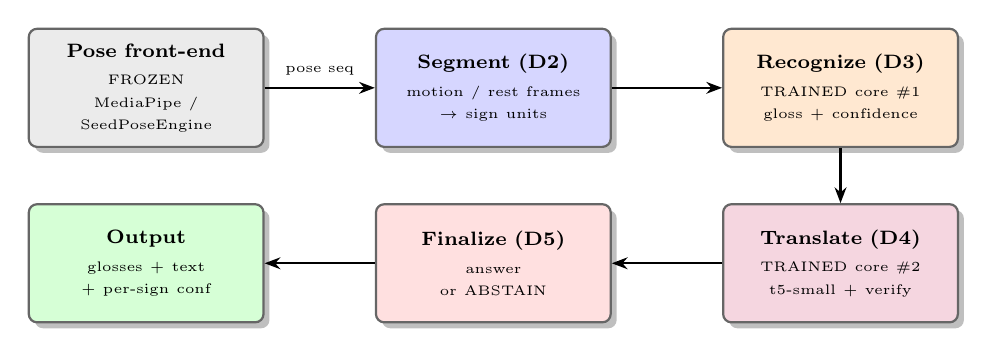
\begin{tikzpicture}[
  node distance=0.7cm and 1.4cm,
  box/.style={rectangle, draw=black!60, rounded corners=3pt, thick,
              text width=2.7cm, minimum height=1.5cm, align=center,
              inner sep=4pt, font=\scriptsize, drop shadow},
  frontbox/.style={box, fill=gray!16},
  segbox/.style={box, fill=blue!16},
  recbox/.style={box, fill=orange!18},
  transbox/.style={box, fill=purple!16},
  finbox/.style={box, fill=red!12},
  arrow/.style={-{Stealth[length=2mm]}, thick}
]

\node[frontbox] (front) {%
  \textbf{Pose front-end}\\[2pt]
  {\tiny FROZEN}\\
  {\tiny MediaPipe / SeedPoseEngine}
};
\node[segbox, right=of front] (seg) {%
  \textbf{Segment (D2)}\\[2pt]
  {\tiny motion / rest frames}\\
  {\tiny $\rightarrow$ sign units}
};
\node[recbox, right=of seg] (rec) {%
  \textbf{Recognize (D3)}\\[2pt]
  {\tiny TRAINED core \#1}\\
  {\tiny gloss + confidence}
};
\node[transbox, below=of rec] (trans) {%
  \textbf{Translate (D4)}\\[2pt]
  {\tiny TRAINED core \#2}\\
  {\tiny t5-small + verify}
};
\node[finbox, left=of trans] (fin) {%
  \textbf{Finalize (D5)}\\[2pt]
  {\tiny answer}\\
  {\tiny or ABSTAIN}
};
\node[box, fill=green!16, left=of fin] (out) {%
  \textbf{Output}\\[2pt]
  {\tiny glosses + text}\\
  {\tiny + per-sign conf}
};

\draw[arrow] (front) -- node[above=1pt, font=\tiny] {pose seq} (seg);
\draw[arrow] (seg) -- (rec);
\draw[arrow] (rec) -- (trans);
\draw[arrow] (trans) -- (fin);
\draw[arrow] (fin) -- (out);

\end{tikzpicture}%
}

\vspace{0.2cm}
\scriptsize Only the \textbf{recognizer} and \textbf{translator} are trained; the pose front-end is frozen/algorithmic and the segmenter is pure geometry. A deterministic FSM (D1 ingest precedes D2) wraps the cascade and decides whether to answer or \textbf{abstain}. Offline: \texttt{SeedPoseEngine} + numpy centroid + lexicon, no torch / mediapipe / network.
\end{frame}

% ============================================================
% SLIDE 6: REPOSITORY & TECH STACK
% ============================================================
\begin{frame}[fragile]{4. Repository Structure \& Tech Stack}
\begin{columns}[T]
\begin{column}{0.55\textwidth}
\textbf{GitHub repo} (public, MIT) \\
\scriptsize \url{https://github.com/ledinhminhquan/01_Sign_Language_Translation}

\vspace{0.1cm}
\begin{lstlisting}[basicstyle=\ttfamily\tiny]
src/signlang/
  pose/         # NET-NEW: layout + engine
  data/         # synth_pose.py (PRIMARY) + lexicon
  segmentation/ # motion-based segmenter (D2)
  models/       # recognizer + translator + baselines
  agent/        # NET-NEW: 5-decision FSM (D1..D5)
  api/          # FastAPI (/translate) + Gradio UI
  analysis/     # WER/BLEU/chrF/boundary-F1
  autoreport/   # auto report PDF + slides
  monitoring/   # drift_report.py
  automation/   # one-button autopilot
  grading/      # rubric self-check (score 1.0)
docs/           # 14 Section-I docs
notebooks/      # Colab H100 autopilot
Dockerfile      # ffmpeg + libGL (video->pose)
\end{lstlisting}
\end{column}
\begin{column}{0.45\textwidth}
\textbf{Tech stack}
\begin{itemize}\small
  \item Python (offline: numpy only)
  \item Git + GitHub (MIT)
  \item \textbf{MediaPipe Holistic} (Apache, frozen)
  \item \textbf{t5-small} (Apache, 60.5M) translator
  \item $\sim$5M transformer / numpy-centroid recognizer
  \item PyTorch + Transformers (Colab)
  \item FastAPI + Uvicorn + Gradio
  \item Docker (ffmpeg + libGL)
  \item Colab T4 (sufficient) / H100 autopilot
\end{itemize}
\scriptsize Every load-bearing model is \textbf{Apache-2.0 / MIT}; no NC / gated dependency anywhere.
\end{column}
\end{columns}
\end{frame}

% ============================================================
% SLIDE 7: DATA MANAGEMENT
% ============================================================
\begin{frame}{5. Data Management -- A License-Clean Synthetic Spine}
\begin{columns}[T]
\begin{column}{0.5\textwidth}
\textbf{Defining constraint (verified on the Hub)}: \emph{every} continuous SLT corpus is \textbf{NC / gated / unspecified}; benchmarks (PHOENIX-2014T, CSL-Daily, YouTube-ASL) are not even Hub repos.

\vspace{0.1cm}
\textbf{Primary data}: synthetic pose generator
\begin{itemize}\small
  \item 2$\times$21 hand + 25 body $\times$ 3 coords (= MediaPipe layout)
  \item 40 glosses, deterministic motion directions
  \item rest frames separate signs; embedded gold
  \item text $\neq$ gloss (\texttt{THANK-YOU}$\rightarrow$``thank you'')
\end{itemize}
\end{column}
\begin{column}{0.5\textwidth}
\textbf{Sources \& licenses (all flagged)}
\begin{table}[h]
\centering\scriptsize
\begin{tabular}{ll}
\toprule
\textbf{Source} & \textbf{License / role} \\
\midrule
\texttt{synth\_pose} & ours -- \textbf{PRIMARY} \\
\texttt{Sigurdur/icelandic-sl} & Apache -- smoke test \\
\texttt{om192006/...keypoints} & MIT -- schema \\
\texttt{How2Sign\_Holistic} & \textbf{FLAG} NC upstream \\
\texttt{Exploration-Lab/iSign} & \textbf{FLAG} NC-SA+gated \\
\texttt{Voxel51/WLASL} & \textbf{FLAG} other \\
\bottomrule
\end{tabular}
\end{table}
\scriptsize \textbf{Honest limit}: synthetic validates the \emph{plumbing} + baseline ordering, not real-language quality (no non-manual features, no signer variation, no real noise).
\end{column}
\end{columns}
\end{frame}

% ============================================================
% SLIDE 8: TRAINING & AUTOPILOT WORKFLOW (TikZ)
% ============================================================
\begin{frame}{6. Training \& Autopilot Workflow}
\centering
\begin{tikzpicture}[
  node distance=0.16cm,
  step/.style={rectangle, draw=black!60, rounded corners=2pt, thick,
              minimum width=11.5cm, minimum height=0.52cm, align=center, font=\scriptsize},
  setup/.style={step, fill=gray!15},
  evalb/.style={step, fill=blue!15},
  train/.style={step, fill=orange!15},
  deploy/.style={step, fill=green!15},
  arrow/.style={-{Stealth[length=1.8mm]}, thick}
]
\node[setup] (s1) {\textbf{1. Offline spine (CPU)}: synth $\rightarrow$ SeedPose $\rightarrow$ segment $\rightarrow$ numpy-centroid $\rightarrow$ lexicon (no torch/mediapipe/net)};
\node[evalb, below=of s1] (s2) {\textbf{2. Offline metrics + 4 baselines}: gloss-WER/acc/EM, BLEU/chrF/WER, boundary-F1, abstention};
\node[setup, below=of s2] (s3) {\textbf{3. Colab setup}: GPU runtime, install \texttt{[all]} extras, mount Drive ~~~\textbf{(hard CPU-green gate above)}};
\node[train, below=of s3] (s4) {\textbf{4. Train recognizer}: compact transformer encoder ($\sim$5M, student-scale)};
\node[train, below=of s4] (s5) {\textbf{5. Train translator}: fine-tune \texttt{t5-small} (gloss$\rightarrow$text), reuse P13/P14 seq2seq pattern};
\node[evalb, below=of s5] (s6) {\textbf{6. Full eval + pose-noise sweep} + real-data smoke test (Icelandic SL, Apache)};
\node[deploy, below=of s6] (s7) {\textbf{7. Auto-gen} report PDF + slides PPTX (with the SLT-metric reliability caveat)};
\node[deploy, below=of s7] (s8) {\textbf{8. Submission bundle} + grading self-check (\textbf{score 1.0})};
\foreach \a/\b in {s1/s2,s2/s3,s3/s4,s4/s5,s5/s6,s6/s7,s7/s8}
  \draw[arrow] (\a) -- (\b);
\end{tikzpicture}

\vspace{0.1cm}
\scriptsize \textbf{One code path, offline or online}: lazy imports + capability probes upgrade each stage in place. Deterministic + byte-for-byte reproducible. Both trainable units fit a single Colab T4.
\end{frame}

% ============================================================
% SLIDE 9: EVALUATION RESULTS
% ============================================================
\begin{frame}{7. Evaluation Results -- Verified Offline (Synthetic Test Split)}
\begin{columns}[T]
\begin{column}{0.52\textwidth}
\textbf{Clean trained core vs floors}
\begin{table}[h]
\centering\scriptsize
\begin{tabular}{llc}
\toprule
\textbf{Metric} & \textbf{Stage} & \textbf{Value} \\
\midrule
Gloss accuracy & recognition & \textbf{1.0} \\
Gloss-WER (S/D/I) & recognition & \textbf{0.0} \\
Sequence exact-match & recognition & \textbf{1.0} \\
Boundary-F1 & segmentation & \textbf{1.0} \\
BLEU-4 (headline) & translation & \textbf{99+} \\
Abstention rate & agent & 0 $\rightarrow$ 1 \\
\bottomrule
\end{tabular}
\end{table}
\scriptsize Floors: most-frequent gloss $\approx$\textbf{0.02}; identity-translate $\approx$\textbf{84} BLEU $\Rightarrow$ lexicon adds $\approx$\textbf{+15} BLEU. Pure-noise input \textbf{abstains}; all 5 decisions fire.

\vspace{0.05cm}
\scriptsize \textbf{Caveat}: clean-synthetic 99+/1.0 are upper bounds on a solvable task, \emph{not} real-world SLT quality.
\end{column}
\begin{column}{0.48\textwidth}
\centering
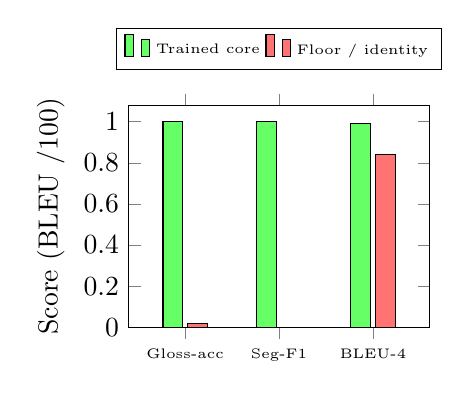
\begin{tikzpicture}
\begin{axis}[
  ybar, width=5.4cm, height=4.4cm,
  ymin=0, ymax=1.08,
  symbolic x coords={Gloss-acc, Seg-F1, BLEU-4},
  xtick=data,
  ylabel={Score (BLEU /100)},
  legend style={font=\tiny, at={(0.5,1.16)}, anchor=south, legend columns=2},
  bar width=7pt,
  enlarge x limits=0.3,
  ytick={0,0.2,0.4,0.6,0.8,1.0},
  x tick label style={font=\tiny}
]
\addplot[fill=green!60] coordinates {(Gloss-acc,1.0) (Seg-F1,1.0) (BLEU-4,0.99)};
\addplot[fill=red!55] coordinates {(Gloss-acc,0.02) (Seg-F1,0.0) (BLEU-4,0.84)};
\legend{Trained core, Floor / identity}
\end{axis}
\end{tikzpicture}\\
\tiny Trained core vs the informed floor / identity baseline (BLEU-4 shown /100).
\end{column}
\end{columns}
\end{frame}

% ============================================================
% SLIDE 10: THE 5-DECISION AGENT (TikZ)
% ============================================================
\begin{frame}{8. Agentic AI -- The 5-Decision Pipeline (D1--D5)}
\centering
\begin{tikzpicture}[
  node distance=0.16cm,
  step/.style={rectangle, draw=black!60, rounded corners=2pt, thick,
              text width=11.4cm, minimum height=0.6cm, align=center, font=\scriptsize,
              inner sep=4pt},
  ingest/.style={step, fill=gray!15},
  seg/.style={step, fill=blue!15},
  rec/.style={step, fill=orange!15},
  trans/.style={step, fill=purple!15},
  fin/.style={step, fill=red!12},
  arrow/.style={-{Stealth[length=2mm]}, thick}
]
\node[ingest] (d1) {\textbf{D1 -- Ingest} (\textbf{decision}): frame-count gate (\texttt{n\_frames$\geq$8}) + route video$\rightarrow$pose / fail};
\node[seg, below=of d1] (d2) {\textbf{D2 -- Segment} (\textbf{reasoning}): low-velocity rest frames (\texttt{q30}) split signs $\rightarrow$ \emph{n} units / single-span};
\node[rec, below=of d2] (d3) {\textbf{D3 -- Recognize} (\textbf{tool}): mean-displacement $\rightarrow$ gloss + conf; $<$\texttt{recog\_min\_conf=0.15} $\rightarrow$ low-conf / OOV};
\node[trans, below=of d3] (d4) {\textbf{D4 -- Translate+verify} (\textbf{tool}): gloss$\rightarrow$text + round-trip chrF keep-gate ($\geq$\texttt{0.20}) / re-flag};
\node[fin, below=of d4] (d5) {\textbf{D5 -- Finalize} (\textbf{decision}): bad-ratio $>$\texttt{oov\_abstain\_ratio=0.50} $\rightarrow$ \textbf{ABSTAIN}; else \textbf{answer}+per-sign conf};
\foreach \a/\b in {d1/d2,d2/d3,d3/d4,d4/d5}
  \draw[arrow] (\a) -- (\b);
\end{tikzpicture}

\vspace{0.1cm}
\scriptsize Satisfies all rubric agentic requirements: \textbf{multi-step reasoning} (D2,D3,D5), \textbf{tool usage} (pose/segment/recognize/translate/verify), \textbf{decision-making} on intermediate outputs (D1,D3,D4,D5). Every state writes a \texttt{ToolTrace} (signal + threshold + branch). Optional \texttt{anthropic} brain is \textbf{OFF by default}, advisory only -- never changes output.
\end{frame}

% ============================================================
% SLIDE 11: AGENT EXAMPLE TRACES
% ============================================================
\begin{frame}[fragile]{9. Agent Example Traces -- Answer vs Abstain}
\textbf{Example 1 -- clean "THANK-YOU ME" (26 frames) $\rightarrow$ ANSWER}
\begin{lstlisting}[basicstyle=\ttfamily\tiny]
D1 ingest:    n_frames=26 >= 8                   -> proceed
D2 segment:   rest run frames 11-13 (3>=2)       -> 2 segments
D3 recognize: THANK-YOU 0.93 ; ME 0.88 (>=0.15)  -> confident
D4 translate: "thank you i" ; roundtrip chrF 0.81 (>=0.20) -> keep
D5 finalize:  bad ratio 0/2 = 0.0 (<=0.50)       -> ANSWER
Output: {"decision":"answer","glosses":["THANK-YOU","ME"],
         "text":"thank you i","per_sign_confidence":[0.93,0.88]}
\end{lstlisting}

\textbf{Example 2 -- pure-noise input $\rightarrow$ ABSTAIN (the value-add)}
\begin{lstlisting}[basicstyle=\ttfamily\tiny]
D1 ingest:    n_frames=30 >= 8                    -> proceed
D2 segment:   no rest run found                   -> single span
D3 recognize: gloss conf 0.04 (< 0.15)            -> low-conf
D4 translate: roundtrip chrF 0.05 (< 0.20)        -> verify_failed
D5 finalize:  bad ratio 1/1 = 1.0 (> 0.50)        -> ABSTAIN
Output: {"decision":"uncertain","text":null,"needs_review":true,
         "note":"Low-confidence signing -- please repeat more slowly."}
\end{lstlisting}

\scriptsize An end-to-end decoder would emit a fluent, confident sentence for the noise input. The agent \textbf{declines}.
\end{frame}

% ============================================================
% SLIDE 12: DEPLOYMENT
% ============================================================
\begin{frame}{10. Deployment (Delivered Capability)}
\textbf{Four deployment formats delivered} (same agent FSM runs inside the handler)
\begin{itemize}\small
  \item \textbf{REST API} (FastAPI): \texttt{GET /healthz}, \texttt{GET /vocabulary}, \texttt{POST /translate}
  \item \textbf{CLI}: \texttt{signlang demo-agent / translate / evaluate / autopilot / grade / train / serve}
  \item \textbf{Docker}: slim image + \texttt{ffmpeg}/\texttt{libGL} for the optional video$\rightarrow$pose path; default = offline Seed profile
  \item \textbf{Gradio demo + Colab autopilot}: interactive UI mounts the same FSM handler
\end{itemize}

\begin{columns}[T]
\begin{column}{0.5\textwidth}
\textbf{Two profiles (config only, no code change)}
\begin{itemize}\small
  \item \textbf{Seed} (default): SeedPose + numpy centroid + lexicon -- \textbf{CPU only}, $\sim$3--10\,ms
  \item \textbf{Full}: MediaPipe + transformer + t5-small -- CPU front-end + \textbf{GPU} core (a T4 is ample)
\end{itemize}
\end{column}
\begin{column}{0.5\textwidth}
\textbf{Honest status}
\begin{itemize}\small
  \item Fully runnable locally / in Docker / on Colab
  \item \textbf{Not} hosted at a live public URL (no Vercel/HF-Space link)
  \item Env-driven config; no secrets in code; \texttt{RETAIN\_INPUTS=0}
\end{itemize}
\end{column}
\end{columns}
\end{frame}

% ============================================================
% SLIDE 13: ETHICS, PRIVACY & FAIRNESS
% ============================================================
\begin{frame}{11. Ethics, Privacy \& Fairness}
\begin{columns}[T]
\begin{column}{0.5\textwidth}
\textbf{Headline position}
\begin{itemize}\small
  \item \textbf{Assistive aid, NOT} a replacement for a qualified human interpreter
  \item Prohibited as sole channel in medical / legal / safety-critical settings
\end{itemize}

\textbf{Privacy (biometric data)}
\begin{itemize}\small
  \item Sign video = face + hands = biometric, identifying, Deaf-community data
  \item On-device / edge processing; \textbf{no retention by default}
  \item LLM brain OFF $\Rightarrow$ no data to a 3rd-party API
  \item Pose keypoints are \emph{not} anonymous (soft biometric)
\end{itemize}
\end{column}
\begin{column}{0.5\textwidth}
\textbf{Representation bias (central risk)}
\begin{itemize}\small
  \item ASL $\neq$ BSL $\neq$ ISL $\neq$ Icelandic SL; heavy within-language variation
  \item A model on one signer/language \textbf{fails on others}
  \item Trained on 40 synthetic ASL-style glosses + a 214-row Icelandic smoke test
  \item Treated as \textbf{unsolved}; never claimed beyond what was evaluated
\end{itemize}

\textbf{The abstention backstop}
\begin{itemize}\small
  \item Surface glosses + per-sign confidence + \texttt{needs\_review}
  \item ``Nothing about us without us'' -- Deaf-community co-design
\end{itemize}
\end{column}
\end{columns}
\end{frame}

% ============================================================
% SLIDE 14: MONITORING & CONTINUAL LEARNING
% ============================================================
\begin{frame}{12. Monitoring \& Continual Learning}
\begin{columns}[T]
\begin{column}{0.5\textwidth}
\textbf{Monitoring} (\texttt{monitoring/drift\_report.py})
\begin{itemize}\small
  \item \textbf{Abstention rate} -- the headline trust metric
  \item Low-confidence segment rate (leading indicator)
  \item Recognition-confidence drift (mean \& p10)
  \item Mean segments/sentence (over/under-split)
  \item D4 verification keep-rate
  \item Pose-extraction quality (Colab/prod)
\end{itemize}
\textbf{Frozen front-end}: we monitor MediaPipe's output, retrain only the recognizer + translator.
\end{column}
\begin{column}{0.5\textwidth}
\textbf{Continual learning loop}
\begin{enumerate}\small
  \item Capture consented, de-identified \emph{pose-only} corrections (abstained cases = gold mine)
  \item Expand the 40-gloss lexicon (OOV is the \emph{normal} case)
  \item Re-fit recognizer (centroid / fine-tune) + refresh t5 translator
  \item Synthetic generator regression-tests new glosses first
  \item Gate on full suite vs baselines + Seed oracle
\end{enumerate}
\scriptsize \textbf{Abstention is the backstop}: a model that scores higher but abstains less on OOV got \emph{worse}. A BLEU bump alone never justifies promotion.
\end{column}
\end{columns}
\end{frame}

% ============================================================
% SLIDE 15: KEY TAKEAWAYS & FUTURE WORK
% ============================================================
\begin{frame}{13. Key Takeaways \& Future Work}
\textbf{Key takeaways}
\begin{itemize}\small
  \item Complete end-to-end SLT cascade: pose $\rightarrow$ segment $\rightarrow$ recognize $\rightarrow$ translate $\rightarrow$ verify $\rightarrow$ \textbf{abstain}
  \item License-honest design: \textbf{no permissive Sign$\rightarrow$Text checkpoint / corpus exists} $\Rightarrow$ train our own small seq2seq on a synthetic spine; every component Apache-2.0 / MIT
  \item Verified offline: gloss accuracy \textbf{1.0}, BLEU \textbf{99+}, segmentation-F1 \textbf{1.0} vs floor 0.02 / identity 84; pure-noise \textbf{abstains}; rubric self-check \textbf{1.0}
  \item Intelligent \textbf{5-decision agent} (reasoning + tools + decisions) whose value is \emph{knowing when not to answer}
  \item Deployable (FastAPI + Gradio + Docker + Colab); runs fully offline on CPU
\end{itemize}

\textbf{Future work}
\begin{enumerate}\small
  \item Active learning from abstained / interpreter-reviewed cases (consented, pose-only)
  \item Larger recognizer + a real continuous corpus under a proper data agreement
  \item Multilingual targets via \texttt{m2m100}; byte-level \texttt{byt5} for fast vocabulary churn
  \item Non-manual features (face / mouthing) for grammatical signal
  \item Token-level explainability + a drift dashboard reading the monitoring logs
\end{enumerate}
\end{frame}

% ============================================================
% SLIDE 16: RESOURCES & THANK YOU (Final slide)
% ============================================================
\begin{frame}{14. Project Resources \& Thank You}
\begin{block}{Source code (public)}
\centering
\large \textbf{\url{https://github.com/ledinhminhquan/01_Sign_Language_Translation}}
\end{block}

\textbf{All public resources}
\begin{itemize}\scriptsize
  \item \textbf{GitHub repo (MIT)}: \tiny\url{https://github.com/ledinhminhquan/01_Sign_Language_Translation}
  \item \textbf{Translator (trained core)}: \tiny\texttt{google-t5/t5-small} (Apache-2.0) -- \url{https://huggingface.co/google-t5/t5-small}
  \item \textbf{Recognizer scale ref}: \tiny\texttt{manohonsy/how2sign-pose-cslr} (MIT, 4.8M)
  \item \textbf{Real-data smoke corpus}: \tiny\texttt{Sigurdur/icelandic-sign-language} (Apache-2.0, 214 rows)
  \item \textbf{Colab autopilot}: \tiny\texttt{notebooks/Sign\_Language\_Translation\_Colab\_H100.ipynb}
\end{itemize}

\vspace{0.2cm}
\centering
\Large\textbf{Thank you for your attention!}\\[0.2cm]
\normalsize Le Dinh Minh Quan -- 23127460 -- 23CNTThuc \\
\small CSC15012 -- Applications of NLP in Industry -- 2026
\end{frame}

\end{document}
